\documentclass[a4paper, 12pt]{article}

%Paragraph jumps and indentation
\setlength{\parskip}{1.4em}
\setlength{\parindent}{1.25cm}

%Border
\usepackage[left=1in, right=1in, top=1in, bottom=1in]{geometry}

%Double spacing
\usepackage{setspace}
\doublespacing

%Packages
\usepackage{amsmath}
\usepackage[dvipsnames]{xcolor}
\usepackage{mathtools}
\usepackage{amsfonts}
\usepackage{titlesec}

%Images
\usepackage{graphicx}
\graphicspath{ {./images/} }
\usepackage{wrapfig}
\usepackage{float}

%Tables
\usepackage{multirow}
\usepackage{array}
\usepackage{tabu}
\titleformat{\section}
{\normalfont\large\bfseries}{\thesection}{1em}{}
\titleformat{\subsection}
{\normalfont\large\bfseries}{\thesubsection}{1em}{}

%Equation numbering
\counterwithin{equation}{section}

%Links
\usepackage{hyperref}
\urlstyle{same}

%Diagrams
\usepackage{pgfplots}
\pgfplotsset{compat = newest}
\usetikzlibrary{positioning, arrows.meta}
\usepgfplotslibrary{fillbetween}
\usepackage{wrapfig}


\begin{document}

\begin{titlepage}
  \begin{center}
    \textbf{IB ECONOMICS} \hspace{1cm} STANDARD LEVEL\\
    \vspace*{3cm}
    \textbf{Title of the article:}
    Yle budget cuts agreed after Left,
    Greens and Finns Party approve new deal\\

    \textbf{Source of the article:}
    Yle News\\

    \textbf{Link to the article:}
    \url{https://yle.fi/a/74-20111279}\\

    \textbf{Article publish date:}
    September 12, 2024\\

    \textbf{Commentary writing date:} \today\\

    \textbf{Unit of the syllabus:}
    Microeconomics\\

    \textbf{Key concept:}
    Economic Well-Being.\\

    \vfill
    Word count: 739
  \end{center}
\end{titlepage}

\section*{Extract}
{ \itshape
  {\large The deal means that Yle faces a funding freeze and an increase in VAT payments, after a long drawn-out battle over setting the company's spending limits up to 2027.}

  Yle faces a years-long funding freeze after parliamentary parties agreed a deal on the company's budget, with the Finns Party, Greens and Left Alliance all approving the new agreement.

  The deal will freeze the budget until 2027, and increase the VAT rates levied on the company from 10 percent to 14 percent from 2026. Yle's budget in 2027 will be around 47 million euros smaller than it would be if index-linked budget increases occurred annually.

  The company will also be obliged to increase commissioning from external production companies, with external purchases slated to be around 15-20 percent higher than they were in the period 2021-2023.

  In addition, Yle will be required to publish more information about its activities and spending.

  The company is owned by the Finnish state and funded by a tax that in 2024 was a maximum of 163 euros per year for individual taxpayers, with reductions for those on lower incomes, or 3,000 euros for businesses.

  Parties have been at loggerheads over Yle's budget since the election campaign, in which both the National Coalition and Finns Party argued for cuts worth more than a hundred million euros in Yle's funding.
}
\newpage
\textbf{\textit{\large Consensus decision}}\\
{ \itshape

  Yle's budget is traditionally decided by cross-party consensus, separate to the government programme. This is regarded as a safeguard against politicising the public service media company, but this time around negotiations were difficult and protracted.

  National Coalition MP Matias Marttinen chaired the working group seeking a compromise, with his own party and the Finns Party suggesting that the government could take the decision themselves if cross-party consensus wasn't reached.

  In July a proposal was accepted by all the parliamentary parties except the Greens and the Left Alliance, who were annoyed at the way the proposal had been negotiated between the Finns Party and National Coalition, rather than between all the parties in the working group.

  The two parties secured small changes to the text of the deal, relating to working conditions of staff and reinforced a commitment to the production of high quality programming for children and young people, and its role as a pillar of general education and a guarantor of equality in educational equality.

  The Movement Now party, a one-man group consisting of Apprentice presenter Harry Harkimo, announced early on that it would reject the agreement on Yle funding.
}

\newpage

\section*{Commentary}

The article celebrates the conclusion of discussions within the government regarding the funding of Yle, the Finnish Public Service Media Company.
Consensus is reached after much deliberation, and consequently the budget of Yle will be reduced both directly, by reducing the direct tax "yleisradiovero" from 163\texteuro\ to 160\texteuro, and indirectly through the funding freeze and the VAT increase.
This commentary aims to analyse the effects of the changes by simplifying the situation and treating it as a reduction of direct provision to the news market by the government.
It will be shown that this change successfully advances \textbf{\color{orange}economic well-being}, around which the discussion will revolve.
To examine the possible effects of this change, we must first know what the situation is prior to the change.

\begin{wrapfigure}{L}{0.6\textwidth}
  \begin{center}
    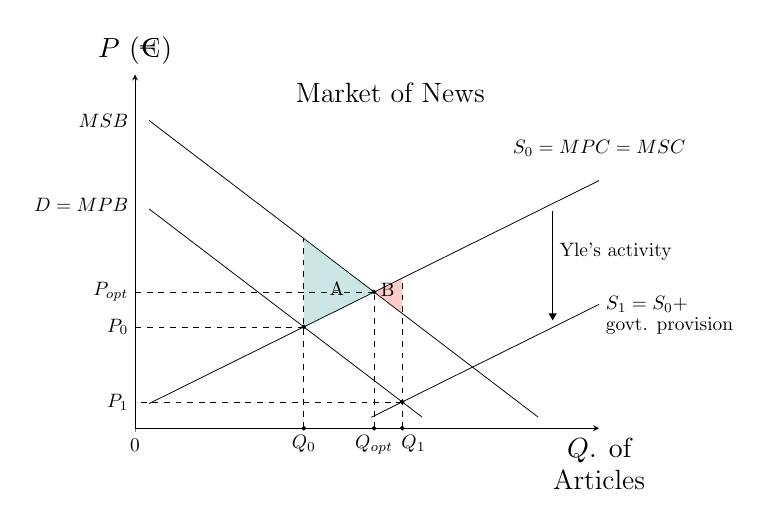
\begin{tikzpicture}[scale=0.7]
      \begin{axis}[
          width=10cm,
          height=8cm,
          axis lines = left,
          xtick = {0},
          ytick = {\empty},
          xmin = 0, xmax = 10,
          ymin = 0, ymax = 10,
          clip = false
        ]
        % Supply curves
        \addplot[domain = 0.3:10, restrict y to domain = 0.3:10, samples = 400]{0.65*x+0.5};
        \addplot[domain = 0.3:10, restrict y to domain = 0.3:10, samples = 400]{0.65*x-3};

        % Demand curves
        \addplot[domain = 0.3:10, restrict y to domain = 0.3:10, samples = 400]{-x+6.5};
        \addplot[domain = 0.3:10, restrict y to domain = 0.3:10, samples = 400]{-x+9};

        % D/S curve labels
        \node[above] at (10, 7.5) {$S_0=MPC=MSC$};
        \node[right] at (10, 3.5) {$S_1=S_0 + $};
        \node[right] at (10, 2.9) {govt. provision};

        \node[left] at (0, 6.3) {$D=MPB$};
        \node[left] at (0, 8.7) {$MSB$};

        \draw[dashed] (5.15152, 0) -- (5.15152, 3.84849);
        \draw[dashed] (0, 3.84849) -- (5.15152, 3.84849);
        \filldraw[black] (5.15152, 3.84849) circle (1pt);
        
        \filldraw[black] (5.15152, 0) circle (1pt);
        \node[below] at (5.15152, 0) {$Q_{opt}$};
        \node[left] at (0, 3.84848) {$P_{opt}$};
        
        \draw[dashed] (3.63636, 0) -- (3.63636, 5.36364);
        \draw[dashed] (3.63636, 2.86364) -- (0, 2.86364);
        \filldraw[black] (3.63636, 2.86364) circle (1pt);
        
        \filldraw[black] (3.63636, 0) circle (1pt);
        \node[below] at (3.63636, 0) {$Q_0$};
        \node[left] at (0, 2.86364) {$P_0$};


        \draw[dashed] (5.75758, 0) -- (5.75758, 4.24243);
        \draw[dashed] (5.75758, 0.74242) -- (0, 0.74242);
        \filldraw[black] (5.75758, 0.74242) circle (1pt);
        
        \filldraw[black] (5.75758, 0) circle (1pt);
        \node[below] at (6, 0) {$Q_1$};
        \node[left] at (0, 0.74242) {$P_1$};
        
        \fill[teal, opacity = 0.2] (3.63636, 2.86364) -- (5.15152, 3.84848) -- (3.63636, 5.36364);
        \node[left] at (4.65152, 3.94848) {A};
        
        \fill[red, opacity = 0.2] (5.75758, 4.24243) -- (5.75758, 3.24242) -- (5.15152, 3.84848);
        \node[right] at (5.15152, 3.89848) {B};

        \draw[-Triangle] (9, 6.15) to (9, 3.05);
        \node[right] at (9, 5) {Yle's activity};

        \node[below] at (10, -1) {\Large Articles};
        \node[above] at (5.5, 9) {\Large Market of News};

      \end{axis}
      \node[below] at (current axis.right of origin) {$Q$. of};
      \node[above] at (current axis.above origin) {$P \text{ (\texteuro)}$};
    \end{tikzpicture}
    \caption{Introducing Yle to Reduce Welfare Loss}
  \end{center}
\end{wrapfigure}

\noindent \textbf{Figure 1} shows the externality that would arise if the Finnish government does not intervene in the news markets through directly providing content with Yle.
The $MSB$ curve lies above $MPB$, because a positive externality of consumption is present.
When Finnish citizens consume news, it makes them more informed, and that produces benefit to the whole society.
When left on its own, the market will create welfare loss equal to size $A$, due to the positive consumption externality. 
In particular, the market equilibrium would be at $Q_0$, which is less than the quantity $Q_{opt}$, the optimum amount of News the Finnish market should provide.
That means an unregulated market forgoes social surplus equal to the area $A$, so that is the amount of welfare loss created by the externality.
The government undertakes direct provision in the News market by creating Yle, whose task is to correct the welfare loss.

The effects of introducing Yle to directly provide news means the supply curve shifts from $S_0$ to $S_1$.
The price and quantity of news settle to new equilibriums $P_1$ and $Q_1$ respectively.
This is good since the welfare loss in this case is only area $B$, which is less than the area $A$ considered previously.
Now we are ready to examine this reduction in Yle's budget.%TODO todo REMOVE THIS ROW IF TOO MANY WORDS.

\begin{wrapfigure}{L}{0.6\textwidth}
  \begin{center}
    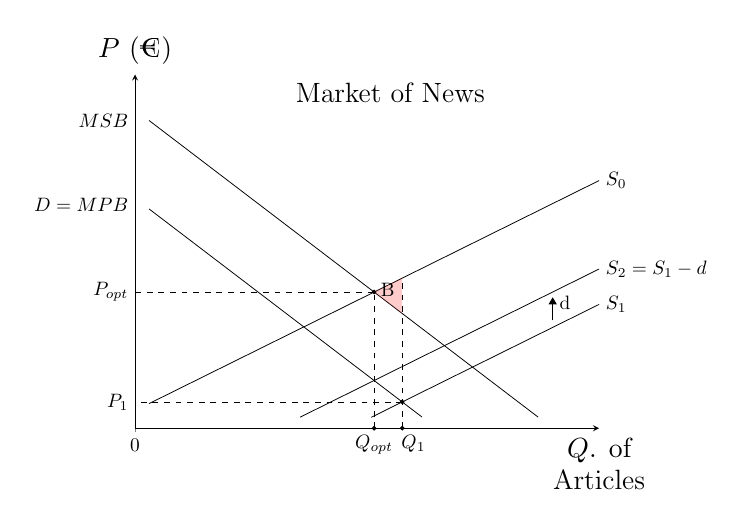
\begin{tikzpicture}[scale=0.7]
      \begin{axis}[
          width=10cm,
          height=8cm,
          axis lines = left,
          xtick = {0},
          ytick = {\empty},
          xmin = 0, xmax = 10,
          ymin = 0, ymax = 10,
          clip = false
        ]
        % Supply curves
        \addplot[domain = 0.3:10, restrict y to domain = 0.3:10, samples = 400]{0.65*x+0.5};
        \addplot[domain = 0.3:10, restrict y to domain = 0.3:10, samples = 400]{0.65*x-3};
        \addplot[domain = 0.3:10, restrict y to domain = 0.3:10, samples = 400]{0.65*x-2};
        % Demand curves
        \addplot[domain = 0.3:10, restrict y to domain = 0.3:10, samples = 400]{-x+6.5};
        \addplot[domain = 0.3:10, restrict y to domain = 0.3:10, samples = 400]{-x+9};

        % D/S curve labels
        \node[right] at (10, 7) {$S_0$};
        \node[right] at (10, 3.5) {$S_1$};
        \node[right] at (10, 4.5) {$S_2=S_1-d$};

        \node[left] at (0, 6.3) {$D=MPB$};
        \node[left] at (0, 8.7) {$MSB$};

        \draw[dashed] (5.15152, 0) -- (5.15152, 3.84849);
        \filldraw[black] (5.15152, 3.84849) circle (1pt);
        
        \filldraw[black] (5.15152, 0) circle (1pt);
        \node[below] at (5.15152, 0) {$Q_{opt}$};
        \node[left] at (0, 3.84848) {$P_{opt}$};

        \draw[dashed] (0, 3.84849) -- (5.15152, 3.84849);
        \draw[dashed] (5.75758, 0) -- (5.75758, 4.24243);
        \draw[dashed] (5.75758, 0.74242) -- (0, 0.74242);
        \filldraw[black] (5.75758, 0.74242) circle (1pt);
        
        \filldraw[black] (5.75758, 0) circle (1pt);
        \node[below] at (6, 0) {$Q_1$};
        \node[left] at (0, 0.74242) {$P_1$};
        
        \fill[red, opacity = 0.2] (5.75758, 4.24243) -- (5.75758, 3.24242) -- (5.15152, 3.84848);
        \node[right] at (5.15152, 3.89848) {B};

        \draw[-Triangle] (9, 3.05) to (9, 3.70);
        \node[right] at (9, 3.55) {d};

        \node[below] at (10, -1) {\Large Articles};
        \node[above] at (5.5, 9) {\Large Market of News};

      \end{axis}
      \node[below] at (current axis.right of origin) {$Q$. of};
      \node[above] at (current axis.above origin) {$P \text{ (\texteuro)}$};
    \end{tikzpicture}
    \caption{Effects of the Budget Cut}
  \end{center}
\end{wrapfigure}

\noindent The budget cut is illustrated in \textbf{Figure 2} as a reduction in the supply of news, by some amount $d$ which we will discuss.
For clarity, the new market equilibrium is shown to settle at the quantity $Q_{opt}$. 
This does, however, not imply that the welfare loss is totally cleared, for the following reasons.

Firstly, the fact that there is a lower quantity or quality of perfectly impartial news supplied by the government means the size of marginal social benefit may shrink by some amount.
This is because other news outlets in the market may be affiliated with political parties.
They also may not be as committed to benefit the population as Yle is, as opposed to maximizing their own financial gains.

In addition, the magnitude of the change may not be as pronounced as the diagram suggests.
This is because the cut is made to the company's budget.
This means that effects are distributed over all of Yle's activities. 
For example, we may expect the company to be producing less sports commentary or entertainment programmes, instead of sacrificing the quantity or quality of news provided.

The speculations above are too vague, and I will use a production possibilities curve (PPC) to obtain a better idea of the specifics.
The article states that the budget will shrink by approximately $47$ million euros, or $\approx 8.6\%$\footnote{The total budget was $547$ million euros in 2024, according to \url{https://yle.fi/a/74-20117417}}.
%Chance to sway the leftist teacher; lefts opposed a large cut.

\begin{wrapfigure}{L}{0.6\textwidth}
  \begin{center}
    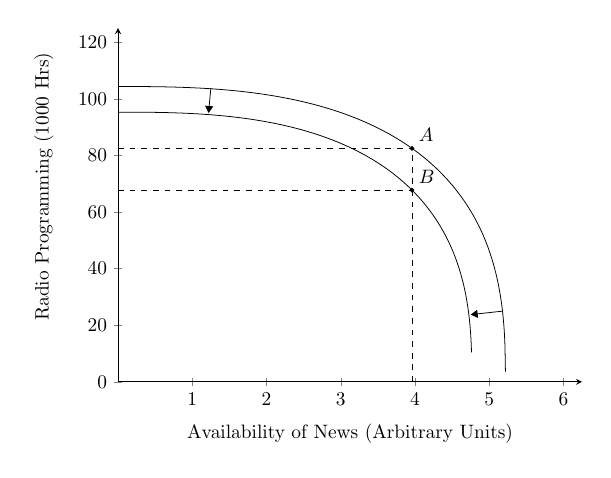
\begin{tikzpicture}[scale=0.7]
      \begin{axis}[
          width=10cm,
          height=8cm,
          axis lines = left,
          xtick={1.6,3.2,...,9.6},
          xticklabels={1,2,...,6},
          ytick={0,1.6,...,9.6},
          yticklabels={0,20,...,120},
          xmin = 0, xmax = 10,
          ymin = 0, ymax = 10,
          clip = false
        ]
        
        \addplot[domain = 0:10, restrict y to domain = 0:10, samples = 1000] {(320-x^2.71828)^0.367879};
        \addplot[domain = 0:10, restrict y to domain = 0:10, samples = 1000] {(250-x^2.71828)^0.367879};

        \draw[-Triangle] (2, 8.3) to (1.95, 7.6);
        \draw[-Triangle] (8.3, 2) to (7.6, 1.9);
        %\draw[-Triangle] (6, 6) to (5.5, 5.4);

        \draw[dashed] (0, 6.6) -- (6.3337, 6.6);
        \draw[dashed] (6.3337, 0) -- (6.3337, 6.6);
        \draw[dashed] (0, 5.42086) -- (6.3337, 5.42086);

        \filldraw[black] (6.3337, 6.6) circle (1pt);
        \node[above right] at (6.3337, 6.6) {$A$};

        \filldraw[black] (6.3337, 5.42086) circle (1pt);
        \node[above right] at (6.3337, 5.42086) {$B$};
        
        \node[below] at (5, -1) {Availability of News (Arbitrary Units)};
        \node[left, rotate=90] at (-1.6, 9.5) {Radio Programming (1000 Hrs)};

      \end{axis}
    \end{tikzpicture}
    \caption{Change in the PPC of Yle}
  \end{center}
\end{wrapfigure}

\noindent \textbf{Figure 3} shows the reduction in Yle's production possibilities, and the choice it must face between producing radio programming and making news available.
We define availability as some metric dependent on the quantity, the quality, and how topical the news is.
The budget cut is displayed as an inwards shift in the PPC curve, as the quantities that Yle is able to produce is now smaller.
In 2023, the amount of radio programming produced is $82210$ hours\footnote{\url{https://yle.fi/aihe/ylen-vuosi-2023}}, as reflected by the diagram.
According to this (rather arbitrary) diagram, that corresponds to a quality of 4 units.
To avoid compromising economic well-being through providing less news, Yle might attempt to keep the amount of news at 4 units.
This means reducing the amount of radio programming to about $69000$ hours.
Note that if this were to be the case, the supply curve $S_1$ from \textbf{Figure 2} would be stationary instead of moving to $S_2$, so $d=0$.
Additionally, the size of the positive consumption externality would not change, so the $MSB$ would also be stationary.



%In addition, a change of this scale is does not risk sacrificing more important factors of economic well-being;
%keeping a wide variety of news and entertainment means the population is able to have a satisfactory level of education both culturally and practically.

%An argument from opposing parties notes that a shortage of content would raise ethical concerns, claiming that the population wishes not to let the quality nor quantity of Yle's content degenerate.
%As a result, only a rather small reduction in Yle's funding is made.
%Although the change succeeds to alleviate the issue of overallocation, it will be shown that a conclusive solution cannot be reached through only adjusting Yle's budget.


\end{document}